%\setcounter{MaxMatrixCols}{30}

\documentclass{article}%
\usepackage{amsmath}
\usepackage{amsfonts}
\usepackage{amssymb}
\usepackage[margin=1in]{geometry}
\usepackage{graphicx}
\usepackage[numbers]{natbib}
\usepackage{cleveref}%
\usepackage{url}
\setcounter{MaxMatrixCols}{30}
%TCIDATA{OutputFilter=latex2.dll}
%TCIDATA{Version=5.50.0.2960}
%TCIDATA{CSTFile=40 LaTeX article.cst}
%TCIDATA{Created=Thursday, January 09, 2025 15:40:48}
%TCIDATA{LastRevised=Friday, March 28, 2025 09:18:44}
%TCIDATA{<META NAME="GraphicsSave" CONTENT="32">}
%TCIDATA{<META NAME="SaveForMode" CONTENT="1">}
%TCIDATA{BibliographyScheme=Manual}
%TCIDATA{<META NAME="DocumentShell" CONTENT="Standard LaTeX\Blank - Standard LaTeX Article">}
%BeginMSIPreambleData
\providecommand{\U}[1]{\protect\rule{.1in}{.1in}}
%EndMSIPreambleData
\newtheorem{theorem}{Theorem}
\newtheorem{acknowledgement}[theorem]{Acknowledgement}
\newtheorem{algorithm}[theorem]{Algorithm}
\newtheorem{axiom}[theorem]{Axiom}
\newtheorem{case}[theorem]{Case}
\newtheorem{claim}[theorem]{Claim}
\newtheorem{conclusion}[theorem]{Conclusion}
\newtheorem{condition}[theorem]{Condition}
\newtheorem{conjecture}[theorem]{Conjecture}
\newtheorem{corollary}[theorem]{Corollary}
\newtheorem{criterion}[theorem]{Criterion}
\newtheorem{definition}[theorem]{Definition}
\newtheorem{example}[theorem]{Example}
\newtheorem{exercise}[theorem]{Exercise}
\newtheorem{lemma}[theorem]{Lemma}
\newtheorem{notation}[theorem]{Notation}
\newtheorem{problem}[theorem]{Problem}
\newtheorem{proposition}[theorem]{Proposition}
\newtheorem{remark}[theorem]{Remark}
\newtheorem{solution}[theorem]{Solution}
\newtheorem{summary}[theorem]{Summary}
\newenvironment{proof}[1][Proof]{\noindent\textbf{#1.} }{\ \rule{0.5em}{0.5em}}



\DeclareMathOperator{\supp}{supp}
\newcommand{\R}{\mathbb{R}}
\newcommand{\E}{\mathbb{E}}
\newcommand{\Prob}{\mathbb{P}}
\newcommand{\dd}{\,\mathrm{d}}
\newcommand{\thetahat}{\hat{\theta}_n}
\newcommand{\thetastar}{\theta^*}
\newcommand{\one}{\boldsymbol{1}}



\begin{document}

\title{Bayes-assisted anytime-valid t-tests and confidence sequences for Gaussian means with unknown variance}
\author{Fran\c{c}ois}
\maketitle

\begin{abstract}

We propose an anytime-valid test of $H_0:\mu=0$ versus $H_1:\mu\neq 0$ for i.i.d.\ normal data with unknown variance, using prior information on the standardized effect size $\delta=\mu/\sigma$. The test mixes a scale-invariant likelihood ratio over a prior on $\delta$ and applies the extended Ville inequality to obtain a valid p-process under arbitrary stopping. When the prior is well specified, the method improves power for alternatives favoured by the prior. For every fixed $n$ and dataset, if the prior has polynomial tails and is centered at $m$, then we show that the time-$n$ p-value converges to the anytime-valid $t$-test p-value as $m\to\infty$. Thus the procedure gains power when the prior is accurate and reverts to the noninformative benchmark under extreme prior-data conflict.

    % Data-prior conflict poses a fundamental challenge in anytime-valid inference; informative priors can yield powerful tests when well-specified, but may produce degenerate or vacuous results under misspecification.
    % To address this, we construct anytime valid p-processes and confidence sequences for the mean of a Gaussian distribution with unknown variance, using scale-invariant likelihood ratios and the method of mixture martingales. We show that for any proper prior, the Ville p-value degenerates to zero and the Ville confidence sequence has diverging volume as the sample Sharpe ratio $\hat{\theta}_n$ tends to infinity. In contrast, by combining the extended Ville inequality with priors having polynomial or exponential tails, we obtain extended p-variables that remain bounded under arbitrary data-prior conflict. Specifically, for polynomial-tail priors (e.g., Student-$t$, Cauchy, horseshoe), the extended p-variable converges to that of the noninformative improper Lebesgue prior as conflict grows. These results extend the bounded-influence prior framework of \cite{Cortinovis2025} from the known-variance to the unknown-variance setting. This is an ongoing work; a full convergence theorem for exponential-tail priors ($\kappa > 0$) remains to be established.
    
    
    % When an informative prior is employed, the resulting procedures are more powerful than noninformative alternatives when prior and data agree, but may become uninformative when they conflict. 
\end{abstract}

keywords: p process; extended Ville inequality; power-law tails; method of mixtures 
\section{Introduction}

Some useful references: \cite{Rouder2009,Lai1976,PerezOrtiz2024,Wang2025,Cortinovis2025}.\medskip

Let $Y_1,Y_2,\ldots$ be i.i.d. $\mathcal N(\mu,\sigma^2)$ and let $\theta^*=\frac{\mu}{\sigma}$, where $\mu\in\mathbb R$ and $\sigma>0$ are unknown. 

\subsection{Anytime-valid testing}

We want to design an anytime-valid test for the (composite) hypothesis 
\begin{align}
H_0:\theta^*=\theta_0 \text{ vs }H_1:\theta^*\neq \theta_0.
\label{eq:tests}
\end{align}
This relies on the construction of a sequence of anytime-valid p-values, or p-process, $(P_{n,\theta_0})_{n\geq 1}$, where $P_{n,\theta_0}:=P_{n,\theta_0}(Y_{1:n})$, that satisfies, for any $\alpha\in (0,1)$
\begin{align}
\mathbb P_{H_0}(\exists n \geq 2 \text{ s.t. } P_{n,\theta_0}\leq \alpha)\leq \alpha.
\label{eq:pprocess}
\end{align}
The test then rejects $H_0$ if $P_{k,\theta_0}\leq \alpha$ for some $k\leq n$. 


\subsection{Confidence sequence}

Using now a family of p-processes $((P_{n,\theta_0})_{n\geq 1})_{\theta_0\in\mathbb R}$, one can obtain a confidence sequence for the parameter $\theta^*$ by inversion of the family of tests \eqref{eq:tests}:
$$
C_{\alpha,n}(Y_{1:n})=\left\{ \theta_0 \mid P_{n,\theta_0}> \alpha\right \}
$$
By the above properties of the p-process (Equation \eqref{eq:pprocess}), the sequence $(C_{\alpha,n}(Y_{1:n}))_{n \geq 1}$ is a confidence sequence, satisfying
$$
\mathbb P(\theta^*  \in C_{\alpha,n}(Y_{1:n}) \text{ for all }n\geq 2)\geq 1-\alpha.
$$


\subsection{Bayes-assisted approach}

Assume that some prior information is available on the unknown parameter $\theta^*$, captured by a probability distribution $\Pi_0$ on $\mathbb R$. We are interested in a procedure that leads to more powerful tests/shorter CS than noninformative methods when the prior agrees with the data, but at the same time whose length remains uniformly bounded in case of data-prior conflict. The setting is similar to that of \cite{Cortinovis2025}, except that here we consider that $\sigma$ is unknown. We will be particularly interest in priors that have Laplace-like or polynomial tails.\medskip

%A closely related problem is to derive an anytime-valid test for testing $H_0: \mu/\sigma=\theta_0$ vs $H_1: \mu/\sigma\neq \theta_0$, where $Y_1,Y_2,\ldots$ be i.i.d. $\mathcal N(\mu,\sigma^2)$, with $\mu$, $\sigma$ unknown, in the presence of prior information on the unknown normalised mean. We want the test to have higher power in case the true normalised mean agrees with the prior, while the power reverts to that of a noninformative prior in case of data prior conflict.

\subsection{(Extended) test martingales and (extended) Ville inequality}

The general construction is of the form:
$$
P_{n,\theta_0} = g_{\theta_0}(M_n(Y_{1:n};\theta_0))
$$
where $M_n(Y_{1:n};\theta_0)$ is an (extended) test martingale/generalised likelihood ratio/Bayes factor with respect to a suitable filtration, and $g_{\theta_0}(c)=1/c$ (Ville's inequality case) or (extended Ville inequality)
$$
g_{\theta_0}(c)=\mathbb E\left[\min(M_2(Y_{1:2},\theta_0)/c,1)     \right].
$$
In both cases Ville's or the extended Ville's inequality guarantee that $(P_{n,\theta_0} )_{n\geq 1}$ is a valid p-process.


\section{Background}




Let $\mathcal F_n$ be the sigma algebra generated by $(\frac{Y_1}{|Y_1|},\frac{Y_2}{|Y_1|},\ldots,\frac{Y_n}{|Y_1|})$. Let $Z_i=\frac{Y_i}{|Y_1|}$. Let $\eta_{n,\theta_0}(z_{1:n})$ be the joint density of $(Z_{1},\ldots,Z_n)$  (which does not depend on $\sigma$) under $H_0$ with respect to the counting$\times$ Lebesgue measure.


  For any $\theta$, $\theta_0$, define
\begin{align}
L_n(y_{1:n};\theta_0,\theta)&=\frac{\eta_{n,\theta}\left(\frac{y_1}{|y_1|},\ldots,\frac{y_n}{|y_1|}\right)}{\eta_{n,\theta_0}\left (\frac{y_1}{|y_1|},\ldots,\frac{y_n}{|y_1|}\right )}\\
&=\frac{\int_0^\infty  f_{n,\theta,\sigma}\left(y_{1:n}\right)\frac{1}{\sigma}d\sigma}{\int_0^\infty  f_{n,\theta_0,\sigma}\left(y_{1:n}\right)\frac{1}{\sigma}d\sigma}\\
&=\frac{h_{\theta,n}(y_{1:n})}{h_{\theta_0,n}(y_{1:n})}
\end{align}
where
$$
h_{\theta,n}(y_{1:n})=e^{-n\theta^2/2}A_n(\theta u_n(y_{1:n}))
$$
with
$$
A_n(z)=\frac{1}{\Gamma(n/2)}\int_0^\infty y^{n/2-1}\exp(-y+z\sqrt{2y})dy=\mathbb E[e^{z R_n}]
$$
with $R_n\sim \chi_n$ follows a chi distribution with $n$ degrees of freedom, and
\begin{align}
u_n(y_{1:n})&=\frac{\sum_{i=1}^n y_i}{\sqrt{\sum_{i=1}^n y_i^2}}\in[-\sqrt{n},\sqrt{n}]\\
&=\frac{n\widehat \theta_n}{\sqrt{(n-1)+n(\widehat\theta_n)^2}}
\end{align}
where $\widehat\theta_n=\frac{\overline Y_n}{S_n}$ is the sample Sharpe ratio.

Then, under $\mathcal N(\mu,\sigma^2)$ with $\mu/\sigma=\theta_0$,  $(L_n(Y_{1:n};\theta_0,\theta))_{n\geq 1}$ is a nonnegative $(\mathcal F_n)$-martingale  (see e.g. equations (5) and (6) in \cite{PerezOrtiz2024} and Corollary 4.6 in \cite{Wang2025}).


\subsection{Mixture construction}


We will consider here the mixture
$$
M_n(y_{1:n};\theta_0)=\int_{\mathbb R} L_n(y_{1:n};\theta_0,\theta)\Pi_0(d\theta)=\frac{\int h_{\theta,n}(y_{1:n})\Pi_0(d\theta)}{h_{\theta_0,n}(y_{1:n})}.
$$

If the prior $\Pi_0$ is proper, $(M_n(Y_{1:n};\theta_0))$ is also a nonnegative martingale; otherwise, it is an extended nonnegative martingale (see \cite{Wang2025}). In the proper prior case, $P_{n,\theta_0}=1/M_n(Y_{1:n};\theta_0)$ defines a p-process by Ville's inequality. 


Define (should explain why we start at 2), for $c>0$, the calibration function
$$
g_{\theta_0}(c)=\mathbb E\left[\min(M_2(Y_{1:2},\theta_0)/c,1)     \right]
$$

Then, by the extended Ville inequality,
$$
C_{\alpha,n}(y_{1:n})=\left \{\theta_0 \mid M_n(y_{1:n};\theta_0)<g_{\theta_0}^{-1}(\alpha)\right \}
$$
is an $1-\alpha$ confidence sequence (starting at $n=2$). Additionally, $P_{n,\theta_0}=g_{\theta_0}(M_n(Y_{1:n};\theta_0))$ defines a p-process.  

\subsection{Examples}
We discuss here various priors used in the literature.

\subsubsection{Improper prior}

$\Pi_0(d\theta)= d\theta$. See \cite[Theorem 2]{Lai1976} and \cite[Theorem 4.1 and Section 4.4]{Wang2025}.


\subsubsection{Local Gaussian prior}

$\Pi_0=\mathcal N(\theta_0,1/c)$
See  \cite[Section 4.5]{Wang2025}, where the classical Ville inequality was used.

Note that in this case, $\Pi_0$ depends on $\theta_0$, so cannot really be interpreted as encapsulating prior information about the parameter of interest.


\subsubsection{Cauchy}

See \cite{Rouder2009} and \cite[Remark 4.6.4]{Wang2025}. Assume $\Pi_0=\text{Cauchy}(0,1)$. This prior was used in the context of Bayes factors.


\section{Objective}

Consider a prior $\Pi_0$ centered at some value $m$. In our context, all the scale-invariant likelihood ratios depend on the data only through $\widehat\theta_n=\frac{\overline Y_n}{S_n}$. The conflict between the data and prior can be measured as $|\widehat\theta_n-m|$.
One objective would be to charaterize the fixed-$n$ conflict regime in terms of the tail behaviour of the prior.
%  show that, for a prior with regularly varying tails, the confidence region for $n\geq 1$  converges to the confidence region under the improper prior as $|\widehat\theta_n-m|\to\infty$ with respect to the Hausdorff distance on subsets of $\mathbb R$; that is, the effect of the prior vanishes in case of data-prior conflict. (then we can slightly generalise this to allow for bounded influence, considering priors with Laplace-like tails). Similarly, for hypothesis testing, we may want to show that the p-value converges to the p-value obtained with an improper prior as the conflict goes to infinity.




\section{Special case of hypothesis test with $\theta_0=0$}

Consider
\[
H_0:\theta^*=0 \qquad \text{vs.}\qquad H_1:\theta^*\neq 0.
\]

Write, for brevity,
\[
u_n=u_n(y_{1:n})=\frac{\sum_{i=1}^n y_i}{\sqrt{\sum_{i=1}^n y_i^2}}
=\frac{n\hat\theta_n}{\sqrt{(n-1)+n\hat\theta_n^2}}\in[-\sqrt n,\sqrt n].
\]
Since $A_n(0)=1$, we have
\[
h_{0,n}(y_{1:n})=e^{-n\cdot 0^2/2}A_n(0)=1.
\]
Therefore, for every $\theta\in\mathbb R$,
\[
L_n(y_{1:n};0,\theta)=h_{\theta,n}(y_{1:n})
=e^{-n\theta^2/2}A_n(\theta u_n).
\]

\subsection{General prior}

Let $\Pi$ be a $\sigma$-finite measure on $\mathbb R$ such that the integral below is finite. The corresponding mixture process is
\begin{equation}\label{eq:Mn-general-zero}
M_n^\Pi(y_{1:n})
=
\int_{\mathbb R} e^{-n\theta^2/2}A_n(\theta u_n)\,\Pi(d\theta).
\end{equation}
If $\Pi$ is proper, $(M_n^\Pi)_{n\ge 1}$ is a nonnegative martingale and hence
\[
P_n^{V,\Pi}(y_{1:n})=\frac{1}{M_n^\Pi(y_{1:n})}
\]
is a valid Ville p-process.

For a general $\sigma$-finite $\Pi$ (in particular for an improper prior), the appropriate anytime-valid p-variable is the extended one
\begin{equation}\label{eq:extended-p-general-zero}
P_n^{E,\Pi}(y_{1:n})=g_\Pi(M_n^\Pi(y_{1:n})),
\qquad
g_\Pi(c)=\E_{0}\!\left[\min\!\left(\frac{M_2^\Pi(Y_{1:2})}{c},1\right)\right],
\end{equation}
where $\E_0$ denotes expectation under $H_0:\theta^*=0$.

\begin{remark}
For the improper prior considered below, the process starts naturally at $n=2$. Indeed, for the Lebesgue prior one gets $M_1^{\mathrm{Leb}}=+\infty$, since $|u_1|=1=\sqrt 1$.
\end{remark}

\subsection{Improper prior $\Pi(d\theta)=d\theta$}

The relevant improper prior here is the Lebesgue measure on $\mathbb R$:
\[
\Pi_{\mathrm{Leb}}(d\theta)=d\theta.
\]
Then
\[
M_n^{\mathrm{Leb}}(y_{1:n})
=
\int_{\mathbb R} e^{-n\theta^2/2}A_n(\theta u_n)\,d\theta.
\]

\begin{proposition}\label{prop:improper-Mn}
For every $n\ge 2$ and every $u\in(-\sqrt n,\sqrt n)$,
\begin{equation}\label{eq:Mn-improper-closed}
M_n^{\mathrm{Leb}}(u)
=
\sqrt{\frac{2\pi}{n}}
\left(1-\frac{u^2}{n}\right)^{-n/2}.
\end{equation}
Equivalently,
\begin{equation}\label{eq:Mn-improper-hattheta}
M_n^{\mathrm{Leb}}(y_{1:n})
=
\sqrt{\frac{2\pi}{n}}
\left(1+\frac{n\hat\theta_n^2}{n-1}\right)^{n/2}.
\end{equation}
\end{proposition}

\begin{proof}
Using the representation $A_n(z)=\E[e^{zR_n}]$ with $R_n\sim\chi_n$, Tonelli's theorem gives
\begin{align*}
M_n^{\mathrm{Leb}}(u)
&=
\int_{\mathbb R} e^{-n\theta^2/2}\E[e^{\theta u R_n}]\,d\theta\\
&=
\E\!\left[\int_{\mathbb R}\exp\!\left(-\frac n2\theta^2+\theta uR_n\right)d\theta\right].
\end{align*}
Completing the square,
\[
-\frac n2\theta^2+\theta uR_n
=
-\frac n2\left(\theta-\frac{uR_n}{n}\right)^2+\frac{u^2R_n^2}{2n},
\]
hence
\[
\int_{\mathbb R}\exp\!\left(-\frac n2\theta^2+\theta uR_n\right)d\theta
=
\sqrt{\frac{2\pi}{n}}\exp\!\left(\frac{u^2R_n^2}{2n}\right).
\]
Therefore
\[
M_n^{\mathrm{Leb}}(u)
=
\sqrt{\frac{2\pi}{n}}\,
\E\!\left[\exp\!\left(\frac{u^2R_n^2}{2n}\right)\right].
\]
Since $R_n^2\sim\chi_n^2$, its mgf is $(1-2t)^{-n/2}$ for $t<1/2$. Taking
$t=u^2/(2n)$ yields \eqref{eq:Mn-improper-closed}. Finally,
\[
1-\frac{u_n^2}{n}
=
\frac{n-1}{(n-1)+n\hat\theta_n^2},
\]
which gives \eqref{eq:Mn-improper-hattheta}.
\end{proof}

For $n=2$, \eqref{eq:Mn-improper-closed} becomes
\begin{equation}\label{eq:M2-improper}
M_2^{\mathrm{Leb}}(u)
=
\sqrt{\pi}\left(1-\frac{u^2}{2}\right)^{-1}
=
\frac{2\sqrt{\pi}}{2-u^2}.
\end{equation}

\begin{proposition}\label{prop:g-improper}
Let
\[
g_{\mathrm{Leb}}(c)
=
\E_0\!\left[\min\!\left(\frac{M_2^{\mathrm{Leb}}(Y_{1:2})}{c},1\right)\right].
\]
Then
\begin{equation}\label{eq:g-improper-explicit}
g_{\mathrm{Leb}}(c)=
\begin{cases}
1, & c\le \sqrt{\pi},\\[0.8em]
\displaystyle
\frac{2}{\pi}
\left[
\arcsin\!\left(\sqrt{\frac{\sqrt\pi}{c}}\right)
+
\sqrt{\frac{\sqrt\pi}{c}\left(1-\frac{\sqrt\pi}{c}\right)}
\right],
& c>\sqrt{\pi}.
\end{cases}
\end{equation}
Hence the improper-prior p-variable is
\begin{equation}\label{eq:p-improper}
P_n^{\mathrm{Leb}}(y_{1:n})
=
g_{\mathrm{Leb}}\!\left(M_n^{\mathrm{Leb}}(y_{1:n})\right).
\end{equation}
\end{proposition}

\begin{proof}
Under $H_0$, let
\[
V=\frac{Y_1+Y_2}{\sqrt 2},
\qquad
W=\frac{Y_1-Y_2}{\sqrt 2}.
\]
Then $V$ and $W$ are independent $\mathcal N(0,\sigma^2)$ random variables, and
\[
1-\frac{U_2^2}{2}
=
\frac{W^2}{V^2+W^2}.
\]
Since $V^2/\sigma^2$ and $W^2/\sigma^2$ are independent $\chi_1^2$, it follows that
\[
B:=1-\frac{U_2^2}{2}\sim \mathrm{Beta}(1/2,1/2),
\qquad
f_B(b)=\frac{1}{\pi\sqrt{b(1-b)}},\quad b\in(0,1).
\]
By \eqref{eq:M2-improper},
\[
M_2^{\mathrm{Leb}}(U_2)=\frac{\sqrt{\pi}}{B}.
\]
Hence
\[
g_{\mathrm{Leb}}(c)
=
\int_0^1 \min\!\left(\frac{\sqrt{\pi}}{cb},1\right)\frac{db}{\pi\sqrt{b(1-b)}}.
\]
If $c\le \sqrt{\pi}$, then $\sqrt{\pi}/(cb)\ge 1$ for all $b\in(0,1)$, hence $g_{\mathrm{Leb}}(c)=1$.

Now assume $c>\sqrt{\pi}$ and put $a=\sqrt{\pi}/c\in(0,1)$. Then
\begin{align*}
g_{\mathrm{Leb}}(c)
&=
\int_0^a \frac{db}{\pi\sqrt{b(1-b)}}
+
a\int_a^1 \frac{db}{\pi b\sqrt{b(1-b)}}\\
&=
\frac{2}{\pi}\arcsin(\sqrt a)
+
\frac{2}{\pi}\sqrt{a(1-a)},
\end{align*}
which is exactly \eqref{eq:g-improper-explicit}.
\end{proof}

\subsection{Recovery of the improper prior for shifted polynomial-tail priors}

Let $\pi$ be a proper density on $\mathbb R$, and for $m\in\mathbb R$ define the location-shifted prior
\[
\pi_m(\theta)=\pi(\theta-m).
\]
Assume that the left tail of $\pi$ is regularly varying:
\begin{equation}\label{eq:poly-tail}
\pi(x)\sim C_-|x|^{-\beta}L(|x|)\qquad \text{as }x\to-\infty,
\end{equation}
for some $\beta>1$, some $C_->0$, and some slowly varying function $L$.
For symmetric priors, this is equivalent to
\[
\pi(x)\sim C|x|^{-\beta}L(|x|)\qquad (|x|\to\infty).
\]
Examples:
\begin{itemize}
\item Student-$t_\nu$: $\beta=\nu+1$;
\item horseshoe location family: $\beta=2$.
\end{itemize}

Define
\[
a_m:=\pi(-m)\sim C_-m^{-\beta}L(m)\qquad (m\to\infty),
\]
and
\begin{equation}\label{eq:Mn-m}
M_{n,m}(u)
:=
\int_{\mathbb R} e^{-n\theta^2/2}A_n(\theta u)\pi_m(\theta)\,d\theta.
\end{equation}
Also define the corresponding extended calibration
\[
g_m(c)
=
\E_0\!\left[\min\!\left(\frac{M_{2,m}(U_2)}{c},1\right)\right].
\]

\begin{theorem}\label{thm:recover-improper}
Fix $n\ge 2$ and $u\in(-\sqrt n,\sqrt n)$. Under \eqref{eq:poly-tail},
\begin{equation}\label{eq:Mn-asymp}
\frac{M_{n,m}(u)}{a_m}\longrightarrow M_n^{\mathrm{Leb}}(u)
\qquad\text{as }m\to\infty.
\end{equation}
Moreover, for every $c>0$,
\begin{equation}\label{eq:g-asymp}
g_m(a_m c)\longrightarrow g_{\mathrm{Leb}}(c)
\qquad\text{as }m\to\infty.
\end{equation}
Consequently, for every fixed realization $y_{1:n}$ such that $|u_n(y_{1:n})|<\sqrt n$,
\begin{equation}\label{eq:p-asymp}
g_m\!\left(M_{n,m}(y_{1:n})\right)
\longrightarrow
g_{\mathrm{Leb}}\!\left(M_n^{\mathrm{Leb}}(y_{1:n})\right)
=
P_n^{\mathrm{Leb}}(y_{1:n}).
\end{equation}
That is, for fixed $n$, the extended p-variable associated with the shifted proper prior converges to the p-variable associated with the improper prior.
\end{theorem}

\begin{proof}
For fixed $u\in(-\sqrt n,\sqrt n)$, the asymptotics of $A_n$ imply that there exist constants
$c_u>0$, $C_u>0$, and an integer $q\ge 0$ such that
\begin{equation}\label{eq:hu-envelope}
h_{\theta,n}(u):=e^{-n\theta^2/2}A_n(\theta u)
\le
C_u(1+|\theta|^q)e^{-c_u\theta^2},
\qquad \theta\in\mathbb R.
\end{equation}
In particular, $h_{\theta,n}(u)$ is integrable, and so is
$(1+|\theta|^r)h_{\theta,n}(u)$ for every $r\ge 0$.

Fix $R>0$. Then
\[
\frac{M_{n,m}(u)}{a_m}
=
\int_{|\theta|\le R} h_{\theta,n}(u)\frac{\pi(\theta-m)}{a_m}\,d\theta
+
\int_{R<|\theta|\le m/2} h_{\theta,n}(u)\frac{\pi(\theta-m)}{a_m}\,d\theta
+
\frac{1}{a_m}\int_{|\theta|>m/2} h_{\theta,n}(u)\pi(\theta-m)\,d\theta.
\]
Since $x\mapsto \pi(-x)$ is regularly varying at $+\infty$, the uniform convergence theorem for regularly varying functions gives
\[
\sup_{|\theta|\le R}\left|\frac{\pi(\theta-m)}{a_m}-1\right|\to 0
\qquad (m\to\infty).
\]
Therefore
\[
\int_{|\theta|\le R} h_{\theta,n}(u)\frac{\pi(\theta-m)}{a_m}\,d\theta
\longrightarrow
\int_{|\theta|\le R} h_{\theta,n}(u)\,d\theta.
\]

Also, again by regular variation, there exists a constant $C_R<\infty$ such that for all large $m$,
\[
\sup_{R<|\theta|\le m/2}\frac{\pi(\theta-m)}{a_m}\le C_R.
\]
Hence
\[
\int_{R<|\theta|\le m/2} h_{\theta,n}(u)\frac{\pi(\theta-m)}{a_m}\,d\theta
\le
C_R\int_{|\theta|>R} h_{\theta,n}(u)\,d\theta.
\]

For the last term, since $\pi(\cdot-m)$ is a probability density,
\[
\frac{1}{a_m}\int_{|\theta|>m/2} h_{\theta,n}(u)\pi(\theta-m)\,d\theta
\le
\frac{\sup_{|\theta|>m/2}h_{\theta,n}(u)}{a_m}.
\]
By \eqref{eq:hu-envelope}, the numerator is exponentially small in $m$, whereas
$a_m$ is only polynomially small. Therefore this term converges to $0$.

Letting first $m\to\infty$ and then $R\to\infty$, we obtain
\[
\frac{M_{n,m}(u)}{a_m}
\longrightarrow
\int_{\mathbb R} h_{\theta,n}(u)\,d\theta
=
M_n^{\mathrm{Leb}}(u),
\]
which proves \eqref{eq:Mn-asymp}.

Now fix $c>0$. Since $|U_2|<\sqrt 2$ almost surely under $H_0$, the first part applied with $n=2$ yields
\[
\frac{M_{2,m}(U_2)}{a_m}\to M_2^{\mathrm{Leb}}(U_2)
\qquad\text{a.s. under }H_0.
\]
Because $0\le \min(M_{2,m}(U_2)/(a_m c),1)\le 1$, bounded convergence implies
\[
g_m(a_m c)
=
\E_0\!\left[\min\!\left(\frac{M_{2,m}(U_2)}{a_m c},1\right)\right]
\longrightarrow
\E_0\!\left[\min\!\left(\frac{M_2^{\mathrm{Leb}}(U_2)}{c},1\right)\right]
=
g_{\mathrm{Leb}}(c),
\]
which is \eqref{eq:g-asymp}.

Finally, let $c_m:=M_{n,m}(y_{1:n})/a_m$ and $c:=M_n^{\mathrm{Leb}}(y_{1:n})$. By \eqref{eq:Mn-asymp}, $c_m\to c$. Since each $g_m$ is decreasing, for every $\varepsilon\in(0,c)$ and all sufficiently large $m$,
\[
g_m(a_m(c+\varepsilon))
\le
g_m(a_m c_m)
\le
g_m(a_m(c-\varepsilon)).
\]
Taking $\liminf$ and $\limsup$, using \eqref{eq:g-asymp}, and then letting $\varepsilon\downarrow 0$ gives
\[
g_m(M_{n,m}(y_{1:n}))
=
g_m(a_m c_m)
\longrightarrow
g_{\mathrm{Leb}}(c)
=
g_{\mathrm{Leb}}(M_n^{\mathrm{Leb}}(y_{1:n})).
\]
This proves \eqref{eq:p-asymp}.
\end{proof}

\begin{remark}
The limit above is a statement about the \emph{extended} p-variable $g_m(M_{n,m})$. In contrast, the raw Ville p-value $1/M_{n,m}$ does \emph{not} have a nondegenerate limit as $m\to\infty$, because
\[
M_{n,m}(u)\sim a_m\,M_n^{\mathrm{Leb}}(u)
\qquad\text{and}\qquad a_m\to 0.
\]
The calibration $g_m$ exactly removes this vanishing tail factor.
\end{remark}




\section{Results}

\subsection{Asymptotics of $A_n$}\label{sec:asymp_An}

\[
A_n(z)=\frac{1}{\Gamma(n/2)}\int_0^\infty y^{n/2-1}\exp(-y+z\sqrt{2y})dy=\mathbb E[e^{z R_n}]
\]

Substitute $r = \sqrt{2y}$, to get,

\begin{align*}
A_n(z)&=\frac{2^{1-n/2}}{\Gamma(n/2)}\,e^{z^2/2}\int_0^\infty r^{n-1}e^{-(r-z)^2/2}\,dr\\
&\sim \frac{2^{1-n/2}\sqrt{2\pi}}{\Gamma(n/2)}\,z^{n-1}\,e^{z^2/2}\qquad\text{as }z\to+\infty.
\end{align*}

The exponent $\phi(r) = -r^2/2 + zr$ has unique maximum at $r = z$ with $\phi(z) = z^2/2$ and $\phi''(z) = -1$.  By Laplace's method,

\[
\int_{0}^\infty r^{n-1} e^{\phi(r)} dr \sim z^{n-1} e^{\phi(z)} \int_{-\infty}^\infty  e^{-u^2/2} du = z^{n-1} e^{z^2/2} \sqrt{2\pi} 
\]

Therefore, $A_n(z) \sim \frac{2^{1-n/2}}{\Gamma(n/2)} \sqrt{2\pi} z^{n-1} e^{z^2/2}$ as $z \longrightarrow \infty$.

As $z\longrightarrow - \infty$, we can write $z = -s$ with $s \longrightarrow + \infty$. Thus,
\[
A_n (-s) = \frac{2^{1-n/2}}{\Gamma(n/2)} e^{s^2/2} \int_{0}^{\infty}  r^{n-1} e^{-sr -r^2/2} dr
\]

For large $s$, the main contribution comes from $r \approx 0$. Set $u = sr$, we get,
\[
A_n(-s) = \frac{2^{1-n/2}}{\Gamma(n/2)} s^{-n} \int_{0}^\infty u^{n-1} e^{-u - u^2/(2s^2)} du 
\]

As $s \longrightarrow \infty$, $e^{-u^2/(2s^2)} \longrightarrow 1$. Hence, by DCT,
\[
\int_{0}^\infty u^{n-1} e^{-u-u^2/(2s^2)} du \longrightarrow \int_{0}^\infty u^{n-1} e^{-u} du = \Gamma(n).
\]

Hence, $A_n(z) \sim \frac{2^{1-n/2}\Gamma(n)}{\Gamma(n/2)} |z|^{-n} $ as $z \longrightarrow -\infty$.

\subsection{Asymptotics of $h_{\theta, n}$ as $u_n \longrightarrow \sqrt{n}$}

For fixed $u \in (0, \sqrt{n})$ and $\theta >0$, as $\theta \longrightarrow \infty$,
\[
h_{\theta,n}(u)=e^{-n\theta^2/2}A_n(\theta u) \sim \frac{2^{1-n/2}\sqrt{2\pi}}{\Gamma(n/2)}\, (\theta u)^{n-1} e^{-\theta^2(n-u^2)/2}
\]

At $u = \sqrt{n}$,

\[
h_{\theta,n}(\sqrt{n}) \sim \frac{2^{1-n/2}\sqrt{2\pi}}{\Gamma(n/2)}\,(\theta\sqrt{n})^{n-1}
\]

\begin{theorem}\label{thm:cs_vol}
    Let $\Pi_0$ be a proper prior on $\mathbb{R}$. For any $n\geq 2$ and $\alpha \in (0,1)$, the volume of the Ville Confidence Sequence (VCS) satisfies,
    \[
    \int_\mathbb{R} \one_{\theta_0 \in C_{\alpha, n}^V (y_{1:n})} d\theta_0 \longrightarrow \infty  \qquad \text{ as } |\hat{\theta}_n| \longrightarrow \infty
    \]
\end{theorem}

\begin{proof}
    We prove the claim for the case $\hat{\theta}_n \longrightarrow +\infty$. The case $\hat{\theta}_n \longrightarrow -\infty$ is identical after replacing $Y_i$ by $-Y_i$ since then $u_n \longrightarrow - \sqrt{n}$ and the same argument applies by symmetry.

Let us recall that,
\[
u_n(y_{1:n})=\frac{\sum_{i=1}^n y_i}{\sqrt{\sum_{i=1}^n y_i^2}}\in[-\sqrt{n},\sqrt{n}]
\]

and that $\hat{\theta}_n \longrightarrow +\infty \implies u_n \longrightarrow \sqrt{n}^{-}$

Also, for $\theta \in \mathbb{R}$ and $u \in (-\sqrt{n}, \sqrt{n})$,
\[
h_{\theta,n}(u)=e^{-n\theta^2/2}A_n(\theta u), \qquad h_n(u) = \int_{\mathbb{R}} h_{\theta,n}(u) \pi_0(\theta)d\theta
\]

The Ville confidence set is,

\[
C_{\alpha, n}^V (y_{1:n}) = \{ \theta_0 \in \mathbb{R}: \frac{h_n(u_n)}{h_{\theta_0, n}(u_n)} \leq \frac{1}{\alpha} \} = \{ \theta_0 \in \mathbb{R}: h_{\theta_0, n}(u_n) \geq \alpha h_n(u_n) \}
\]

Thus it suffices to prove that, as $u_n \uparrow \sqrt{n}$, the set $\{\theta_0 \in \mathbb{R}: h_{\theta_0, n}(u_n) \geq \alpha h_n(u_n) \}$ has Lebesgue measure tending to $+\infty$.

Since $h_n(u_n)$ is an average of $h_{\theta_0, n}(u_n)$ under any prior, we have $h_{ n}(u_n) \leq \sup_{\theta \in \mathbb{R}} h_{\theta, n}(u_n)$.

Hence it is enough to show that the $\alpha$-superlevel set of $\theta \mapsto h_{\theta, n} (u_n)$ relative to its own maximum has diverging length.

Let us define $m_n = \sup_{\theta \in \mathbb{R}} h_{\theta, n}(u_n)$. Then, 
$$\{\theta: h_{\theta, n}(u_n) \geq \alpha m_n \} \subseteq \{\theta: h_{\theta_0, n}(u_n) \geq \alpha h_n(u_n) \} = C_{\alpha, n}^V(y_{1:n}).$$ 

So, it is enough to prove that $\lambda(\{\theta: h_{\theta, n}(u_n) \geq \alpha m_n \}) \longrightarrow \infty$, where $\lambda$ denotes the Lebesgue measure.

\textbf{Case 1: $u \leq \sqrt{n} - \delta$}

Fix \(\delta\in(0,\sqrt n)\). If \(u\le \sqrt n-\delta\), then
\[
\gamma(u):=n-u^2 \ge n-(\sqrt n-\delta)^2 = 2\sqrt n\,\delta-\delta^2 >0.
\]
By the large-\(z\) asymptotic,
\[
A_n(z)\sim c_n z^{\,n-1}e^{z^2/2}\qquad \text{as }z\to+\infty,
\]
for a constant \(c_n>0\), hence for \(\theta\to+\infty\),
\[
h_{\theta,n}(u)
=
e^{-n\theta^2/2}A_n(\theta u)
\sim
c_n (\theta u)^{n-1} e^{-\theta^2(n-u^2)/2}
=
c_n (\theta u)^{n-1} e^{-\gamma(u)\theta^2/2}.
\]
Therefore, once \(u\le \sqrt n-\delta\), there exist constants \(C_\delta,c_\delta>0\) such that for all sufficiently large \(\theta>0\),
\[
h_{\theta,n}(u)\le C_\delta (1+\theta^{n-1})e^{-c_\delta\theta^2}.
\]

Moreover, for \(\theta\to-\infty\), since \(A_n(\theta u)=O(|\theta|^{-(n+1)})\), so \(h_{\theta,n}(u)\to0\) as \(\theta\to-\infty\). It follows that for each fixed \(u\le \sqrt n-\delta\), the function \(\theta\mapsto h_{\theta,n}(u)\) is continuous, tends to \(0\) at both tails, and has finite superlevel sets.

This shows that away from the boundary, no blow-up of the confidence-set volume can occur. Therefore the only possible source of divergence is the boundary regime \(u\uparrow\sqrt n\).

Since \(\hat\theta_n\to+\infty\) implies \(u_n\to\sqrt n\), for every fixed \(\delta>0\) we have
\[
u_n>\sqrt n-\delta
\]
for all sufficiently large \(n\) along the given data sequence. So eventually we are in the boundary layer.

\textbf{Case 2: Boundary}\\
Let $\gamma_n:=n-u_n^2$. Then \(\gamma_n>0\) and \(\gamma_n\to0\) as \(u_n\uparrow\sqrt n\).

The expansion of \(A_n\) implies the following two-sided bound, there exist constants
\[
z_0>0,\qquad 0<c_-<c_+<\infty
\]
such that for all \(z\ge z_0\),
\[
c_- z^{n-1}e^{z^2/2}\le A_n(z)\le c_+ z^{n-1}e^{z^2/2}.
\]
Since \(u_n\to\sqrt n>0\), there exists \(N_0\) such that for all large \(n\) along the sequence,
\[
u_n\ge \frac{\sqrt n}{2}.
\]
Hence, for all such indices and all \(\theta\ge 2z_0/\sqrt n\), we have \(\theta u_n\ge z_0\), and therefore
\begin{equation}\label{eq_sandwich}
c_1\, \theta^{n-1} e^{-\gamma_n\theta^2/2}
\;\le\;
h_{\theta,n}(u_n)
\;\le\;
c_2\, \theta^{n-1} e^{-\gamma_n\theta^2/2},
\end{equation}
for suitable constants \(c_1,c_2>0\) depending only on \(n\).

Thus, in the boundary, the value of \(h_{\theta,n}(u_n)\) for positive \(\theta\) is controlled by
\[
\theta\mapsto \theta^{n-1} e^{-\gamma_n\theta^2/2}.
\]
Now that we know the limiting case both in the interior and on the boundary, let us define,
\[
x=\sqrt{\gamma_n}\,\theta,
\qquad \theta=\frac{x}{\sqrt{\gamma_n}}.
\]
Then,
\[
h_{x/\sqrt{\gamma_n},\,n}(u_n)
\asymp
\gamma_n^{-(n-1)/2}\, x^{n-1}e^{-x^2/2},
\]
uniformly for \(x\) in compact subsets of \((0,\infty)\). More precisely, for every compact \(K\subset(0,\infty)\),
\begin{equation}\label{eq_unif}
\gamma_n^{(n-1)/2} h_{x/\sqrt{\gamma_n},\,n}(u_n)
\to
C\, x^{n-1}e^{-x^2/2}
\quad\text{uniformly for }x\in K,
\end{equation}
where
\[
C=c_n (\sqrt n)^{\,n-1}>0   \qquad  c_n = \frac{2^{1-n/2} \sqrt{2\pi}}{\Gamma(n/2)}.
\]

Define
\[
\psi(x):=x^{n-1}e^{-x^2/2},\qquad x>0.
\]
This is continuous, strictly positive on \((0,\infty)\), tends to \(0\) both as \(x\downarrow0\) and as \(x\to\infty\), and has a unique maximizer at
\[
x_*=\sqrt{n-1}.
\]
Let
\[
M_*:=\psi(x_*)>0.
\]

Choose a number \(\eta\) such that
\[
\alpha<\eta<1.
\]
By continuity of \(\psi\) at its strict maximizer \(x_*\), there exist numbers
\[
0<a<x_*<b<\infty
\]
such that
\[
\psi(x)\ge \eta M_*
\qquad\text{for all }x\in[a,b].
\]
Also, since \(\psi(x)\to0\) at \(0\) and \(\infty\), there exist \(0<A<a<b<B<\infty\) such that
\begin{equation}\label{eq_limit}
\sup_{x\notin[A,B]}\psi(x)\le \frac{\eta}{4}M_*.
\end{equation}

By the uniform convergence in~\eqref{eq_unif}, for all sufficiently large indices along the sequence, we have,
\begin{equation}\label{eq_lim_lower}
\gamma_n^{(n-1)/2} h_{x/\sqrt{\gamma_n},\,n}(u_n)
\ge \frac{\eta}{2} C M_*
\qquad\text{for all }x\in[a,b],
\end{equation}
and
\begin{equation}\label{eq_lim_upper}
\gamma_n^{(n-1)/2} h_{x/\sqrt{\gamma_n},\,n}(u_n)
\le \frac{3}{2} C M_*
\qquad\text{for all }x\in[A,B].
\end{equation}

Now let us consider \(\theta\) outside the scaled window \([A/\sqrt{\gamma_n},B/\sqrt{\gamma_n}]\).

\begin{itemize}
\item If \(0\le \theta \le A/\sqrt{\gamma_n}\), then either \(\theta\) remains bounded, in which case \(h_{\theta,n}(u_n)=O(1)\), or else \(x=\sqrt{\gamma_n}\theta\in(0,A]\), in which case~\eqref{eq_unif} and~\eqref{eq_limit} imply
\[
h_{\theta,n}(u_n)\le \frac{\eta}{2} C M_*\,\gamma_n^{-(n-1)/2}
\]
for large indices.

\item If \(\theta \ge B/\sqrt{\gamma_n}\), then \(x\ge B\), and~\eqref{eq_sandwich} together with~\eqref{eq_unif} gives
\[
h_{\theta,n}(u_n)\le \frac{\eta}{2} C M_*\,\gamma_n^{-(n-1)/2}
\]
for large indices.

\item If \(\theta<0\), then since \(u_n>0\), we have \(\theta u_n\to -\infty\) as \(\theta\to-\infty\), and 
\[
A_n(\theta u_n)=O(|\theta|^{-(n+1)}),
\]
so \(h_{\theta,n}(u_n)\) is bounded on \((-\infty,0]\), hence negligible compared to \(\gamma_n^{-(n-1)/2}\to\infty\).
\end{itemize}

Therefore the global maximum \(m_n\) satisfies
\[
m_n\le 2 C M_*\,\gamma_n^{-(n-1)/2}
\]
for all sufficiently large indices, while~\eqref{eq_lim_lower} shows that on the interval
\[
I_n:=\Bigl[\frac{a}{\sqrt{\gamma_n}},\, \frac{b}{\sqrt{\gamma_n}}\Bigr]
\]
we have
\[
h_{\theta,n}(u_n)\ge \frac{\eta}{2} C M_*\,\gamma_n^{-(n-1)/2}.
\]
Choosing the earlier \(\eta\) sufficiently close to \(1\), and then taking the index large enough, we obtain
\[
h_{\theta,n}(u_n)\ge \alpha\, m_n
\qquad\text{for all }\theta\in I_n.
\]
Hence
\[
I_n\subseteq \{\theta:\ h_{\theta,n}(u_n)\ge \alpha m_n\}\subseteq C^V_{\alpha,n}(y_{1:n}).
\]

The length of \(I_n\) is
\[
\lambda(I_n)=\frac{b-a}{\sqrt{\gamma_n}}.
\]
Since \(\gamma_n=n-u_n^2\to0\),
\[
\lambda(I_n)\to\infty.
\]
Because \(I_n\subseteq C^V_{\alpha,n}(y_{1:n})\), it follows that
\[
\lambda\bigl(C^V_{\alpha,n}(y_{1:n})\bigr)\to\infty.
\]

This proves the theorem when \(\hat\theta_n\to+\infty\). The case \(\hat\theta_n\to-\infty\) is symmetric. Therefore
\[
\int_{\mathbb R}\mathbf 1\{\theta_0\in C^V_{\alpha,n}(y_{1:n})\}\,d\theta_0 \to \infty
\qquad\text{as }|\hat\theta_n|\to\infty.
\]
\end{proof}

\section{Calibration function}

For $\kappa \in \mathbb{R}$, we take the improper prior, 
\[
\Pi_0(\theta) = \frac{1}{\sqrt{2\pi \sigma^2}} \exp(-\kappa(\theta - \theta_0)/\sigma) 
\]
To find the marginal likelihood, we integrate the likelihood against our improper prior 

\[
h_{n, \kappa}(u_n) = \int_{-\infty}^\infty e^{-\kappa(\theta - \theta_0) e^{-n\theta^2/2}} A_n(\theta u_n) d\theta
\]

Let us substitute $A_n(\theta u_n) = \E_{\mathbb{R}_n}[e^{\theta u_n R_n}]$ into the integral. By Fubini's theorem, we can swap the integral and the expectation,

\[
h_{n, \kappa}(u_n) = e^{\kappa\theta_0} \E_{R_n} [\int_{-\infty}^\infty \exp(-\frac{n}{2} \theta^2 + \theta(u_nR_n - \kappa))d\theta ]
\]

Now, we complete the square for $\theta$ inside the exponent

\[
-\frac{n}{2} \theta^2 + \theta(u_nR_n - \kappa) = -\frac{n}{2}( \theta - \frac{u_nR_n - \kappa}{n} )^2 + \frac{(u_nR_n - \kappa)^2}{2n}
\]
Thus,
\begin{align*}
    h_{n, \kappa}(u_n) & = e^{\kappa\theta_0} \E_{R_n} [\int_{-\infty}^\infty \exp ( -\frac{n}{2}( \theta - \frac{u_nR_n - \kappa}{n} )^2 + \frac{(u_nR_n - \kappa)^2}{2n}) d\theta ] \\
    & = \sqrt{\frac{2\pi}{n}} e^{\kappa\theta_0} \E_{R_n} [ \exp( \frac{(u_nR_n - \kappa)^2}{2n})] 
\end{align*}

The test martingale is the ratio of the marginal likelihood to the null likelihood 
\begin{align*}
    M_n(U_n, \theta_0) & = \frac{h_{n, \kappa}(u_n)}{h_{\theta_0, n}(u_n)}\\
    & = \frac{\sqrt{\frac{2\pi}{n}} e^{\kappa\theta_0} \E_{R_n} [ \exp( \frac{(u_nR_n - \kappa)^2}{2n})]}{\E_{R_n}[e^{\theta_0 u_n R_n}]}
\end{align*}
According to the extended Ville inequality, the calibration function is evaluated at $n=2$ (since scale invariance requires at least 2 samples)
$$g_{\theta_0}(c) = \mathbb{E}_{U_2 \sim P_{\theta_0}} \left[ \min\left( \frac{M_2(U_2; \theta_0)}{c}, 1 \right) \right]$$

Plugging $n=2$ into our martingale gives
$$M_2(U_2; \theta_0) = \frac{\sqrt{\pi} e^{\kappa\theta_0 + \theta_0^2} \mathbb{E}_{R_2} \left[ \exp\left( \frac{(U_2 R_2 - \kappa)^2}{4} \right) \right]}{\mathbb{E}_{R_2}[ e^{\theta_0 U_2 R_2} ]}$$

If we take the hypothesis as $H_0: \theta_0 = 0$ vs $H_1: \theta_0 \neq 0$, then $e^{\kappa\theta_0 + \theta_0^2} = 1$ and $\mathbb{E}_{R_2}[e^0] = 1$. 

Thus, 
$$\tilde{g}_\kappa(c) = \mathbb{E}_{U_2 \sim P_0} \left[ \min\left( \frac{\sqrt{\pi} \mathbb{E}_{R_2} \left[ \exp\left( \frac{(U_2 R_2 - \kappa)^2}{4} \right) \right]}{c}, 1 \right) \right]$$

\textbf{Case 1: $\kappa = 0$}
$$M_2(u_2; 0) = \mathbb{E}_{R_2} \left[ \exp\left( \frac{u_2^2 R_2^2}{4} \right) \right]$$
where $R_2 \sim \chi_2$ i.e. $f_{R_2}(r) = r e^{-r^2/2} \quad \text{for } r > 0$.
Now,
\begin{align*}
    E = \mathbb{E}_{R_2} \left[ \exp\left( \frac{u_2^2 R_2^2}{4} \right) \right] &  = \int_{0}^{\infty} \exp\left( \frac{u_2^2 r^2}{4} \right) r e^{-r^2/2} dr\\
& = \int_{0}^{\infty} r \exp\left( -r^2 \left( \frac{1}{2} - \frac{u_2^2}{4} \right) \right) dr\\
& = \int_{0}^{\infty} r \exp\left( -r^2 \left( \frac{2 - u_2^2}{4} \right) \right) dr
\end{align*}
Let $v = r^2 \left( \frac{2 - u_2^2}{4} \right)$. Taking the derivative gives $dv = 2r \left( \frac{2 - u_2^2}{4} \right) dr = r \left( \frac{2 - u_2^2}{2} \right) dr$. Rearranging for $r dr$ gives $r dr = \frac{2}{2 - u_2^2} dv$. Hence,
\begin{align*}
    E & = \int_{0}^{\infty} e^{-v} \left( \frac{2}{2 - u_2^2} \right) dv\\
    & = \frac{2}{2 - u_2^2} \int_{0}^{\infty} e^{-v} dv\\
    & = \frac{2}{2 - u_2^2}
\end{align*}
Thus, we get 
$$M_2(u_2; 0) = \frac{2\sqrt{\pi}}{2 - u_2^2}$$
Hence,
$$\tilde{g}_0(c) = \mathbb{E}_{U_2} \left[ \min\left( \frac{2\sqrt{\pi}}{c(2 - U_2^2)}, 1 \right) \right].$$ 

Now, $U_2 = \frac{Y_1 + Y_2}{\sqrt{Y_1^2 + Y_2^2}}$ and hence, $2 - U_2^2 = \frac{(Y_1 - Y_2)^2}{Y_1^2 + Y_2^2}$. So, the denominator $(2 - U_2^2)$ only hits zero if $Y_1 = Y_2$. Since $Y_1$ and $Y_2$ are independent Gaussian random variables, they are continuous; the probability that they take the exact same value is a set of measure zero ($\mathbb{P}(Y_1 = Y_2) = 0$).


\section{$\kappa \neq 0$}

The joint prior on $(\theta, \sigma)$ is
\begin{equation}
  \pi(\theta, \sigma)\, \mathrm{d}\theta\, \mathrm{d}\sigma
  \;=\;
  \frac{\exp\!\bigl(-\kappa(\theta - \theta_0)\bigr)}{\sqrt{2\pi}\, \sigma}\,
  \mathrm{d}\theta\, \mathrm{d}\sigma,
  % \label{eq:kappa:joint-prior}
\end{equation}


Marginal likelihood
\begin{equation}
  M_n^{(\kappa)}(y_{1:n})
  \;=\;
  \int_0^\infty\!\!\int_{\mathbb{R}}
  f_{n, \theta, \sigma}(y_{1:n})\, \pi(\theta, \sigma)\,
  \mathrm{d}\theta\, \mathrm{d}\sigma.
  \label{eq:kappa:Mn-def_2}
\end{equation}


Parabolic cylinder function
(\url{https://en.wikipedia.org/wiki/Parabolic_cylinder_function#Integral_representation})


\begin{proposition}
For every $n \geq 2$ and every $y_{1:n}$ with $u_n \in
(-\sqrt n, \sqrt n)$, the marginal likelihood
\eqref{eq:kappa:Mn-def_2} equals
\begin{equation}
  \;
  M_n^{(\kappa)}(y_{1:n})
  \;=\;
  \frac{(n - 1)!}{(2\pi)^{n/2}\sqrt{n}}\,
  \Bigl(\frac{T_n (n - u_n^2)}{n}\Bigr)^{-n/2}\,
  e^{\Lambda_n(\kappa, u_n)}\,
  D_{-n}\!\Bigl( z_n(\kappa, u_n) \Bigr),
  \;
  \label{eq:kappa:Mn-closed_2}
\end{equation}
where $D_{-n}$ is the parabolic cylinder function, and
\begin{align}
  z_n(\kappa, u_n)
  &\;=\;
  \frac{\kappa\, u_n}{\sqrt{n(n - u_n^2)}},
  \label{eq:kappa:zn_2}
  \\[0.3em]
  \Lambda_n(\kappa, u_n)
  &\;=\;
  \kappa\, \theta_0
  \;+\;
  \frac{\kappa^2}{2n}
  \;+\;
  \frac{\kappa^2 u_n^2}{4 n (n - u_n^2)}.
  \label{eq:kappa:Lambda_2}
\end{align}
Equivalently, using the notation $\hat\theta_n = \bar y_n / S_n^*$,
\[
  z_n(\kappa, u_n) \;=\;
  \frac{\kappa\, \hat\theta_n}{\sqrt{(n-1)/n + \hat\theta_n^2}}\,
  \cdot\, \frac{1}{\sqrt n}.
\]
\end{proposition}


\begin{proof}
The joint prior is
\begin{equation}
  \pi(\theta, \sigma)\, \mathrm{d}\theta\, \mathrm{d}\sigma
  \;=\;
  \frac{\exp\!\bigl(-\kappa(\theta - \theta_0)\bigr)}{\sqrt{2\pi}\, \sigma}\,
  \mathrm{d}\theta\, \mathrm{d}\sigma.
  \label{eq:kappa:joint-prior_2}
\end{equation}
Substituting the likelihood and the
joint prior into
\eqref{eq:kappa:Mn-def_2}, and expanding the squared term as
\[
  \sum_{i=1}^n (y_i - \theta \sigma)^2
  \;=\; T_n - 2 \theta \sigma S_n + n \theta^2 \sigma^2,
\]
the combined exponent in the integrand is
    \begin{align*}
  -\frac{1}{2\sigma^2} \sum_{i=1}^n (y_i - \theta\sigma)^2
  \,-\, \kappa(\theta - \theta_0)
  &\;=\;
  \kappa \theta_0
  \;-\; \frac{T_n}{2\sigma^2}
  \;+\; \theta\, \frac{S_n}{\sigma}
  \;-\; \frac{n \theta^2}{2}
  \;-\; \kappa \theta \\
  &\;=\;
  \kappa \theta_0
  \;-\; \frac{T_n}{2\sigma^2}
  \;+\; \theta\!\left(\frac{S_n}{\sigma} - \kappa\right)
  \;-\; \frac{n \theta^2}{2}.
\end{align*}

The terms involving $\theta$ are
\begin{align*}
  \theta\!\left(\frac{S_n}{\sigma} - \kappa\right)
  - \frac{n}{2} \theta^2
  &\;=\;
  -\frac{n}{2}\!\left(\theta - \frac{1}{n}\!\left(\frac{S_n}{\sigma}
                                                 - \kappa\right)\!\right)^2
  \;+\; \frac{1}{2n}\!\left(\frac{S_n}{\sigma} - \kappa\right)^2.
\end{align*}

The Gaussian integral in $\theta$ over $\mathbb{R}$ gives
$\sqrt{2\pi/n}$, so
\begin{align}
  M_n^{(\kappa)}
  \;=\;
  \frac{e^{\kappa \theta_0}}{(2\pi)^{(n+1)/2}}\,
  \sqrt{\frac{2\pi}{n}}
  \;\int_0^\infty
  \sigma^{-(n+1)}
  \exp\!\Bigl(
    -\frac{T_n}{2\sigma^2}
    + \frac{1}{2n}\!\left(\frac{S_n}{\sigma} - \kappa\right)^2
  \Bigr)\, \mathrm{d}\sigma.
  \label{eq:kappa:after-theta_2}
\end{align}
The total power of $\sigma$ in the integrand is $\sigma^{-(n+1)}$:
$\sigma^{-n}$ from the Gaussian likelihood
$(2\pi\sigma^2)^{-n/2}$, and $\sigma^{-1}$ from the joint prior
\eqref{eq:kappa:joint-prior_2}.  The constant prefactor simplifies via
\[
  \frac{1}{(2\pi)^{(n+1)/2}}\, \sqrt{\frac{2\pi}{n}}
  \;=\;
  \frac{1}{(2\pi)^{n/2} \sqrt n}.
\]

Expanding the squared bracket inside the exponent of
\eqref{eq:kappa:after-theta_2},
\begin{align*}
  -\frac{T_n}{2\sigma^2}
  + \frac{1}{2n}\!\left(\frac{S_n}{\sigma} - \kappa\right)^2
  &\;=\;
  -\frac{T_n}{2\sigma^2}
  + \frac{S_n^2}{2n\sigma^2}
  - \frac{\kappa S_n}{n \sigma}
  + \frac{\kappa^2}{2n}.
\end{align*}
The $\sigma^{-2}$ terms combine to
\[
  -\frac{T_n}{2\sigma^2} + \frac{S_n^2}{2n\sigma^2}
  \;=\;
  -\frac{nT_n - S_n^2}{2n\sigma^2}
  \;=\;
  -\frac{T_n(n - u_n^2)}{2n\sigma^2},
\]
where we used $S_n^2 = u_n^2\, T_n$.  The cross-term, again via
$S_n = u_n \sqrt{T_n}$, becomes
\[
  -\frac{\kappa S_n}{n\sigma}
  \;=\;
  -\frac{\kappa u_n \sqrt{T_n}}{n\sigma}.
\]
Defining
\begin{equation}
  \alpha \;=\; \frac{T_n(n - u_n^2)}{2n} \;>\; 0,
  \qquad
  \beta \;=\; \frac{\kappa u_n \sqrt{T_n}}{n},
  \label{eq:kappa:alpha-beta_2}
\end{equation}
we obtain
\begin{equation}
  M_n^{(\kappa)}
  \;=\;
  \frac{e^{\kappa \theta_0 + \kappa^2/(2n)}}{(2\pi)^{n/2}\sqrt n}\,
  \int_0^\infty \sigma^{-(n+1)}
  \exp\!\Bigl(-\frac{\alpha}{\sigma^2} - \frac{\beta}{\sigma}\Bigr)\,
  \mathrm{d}\sigma.
  \label{eq:kappa:sigma-integral-1_2}
\end{equation}
Crucially, the $\sigma^{-1}$ term $-\beta/\sigma$ in the exponent is
absent in the $\kappa = 0$ case treated in Section~4; this is the
single feature that prevents \eqref{eq:kappa:sigma-integral-1_2} from
reducing to a pure Gamma integral.


Substitute $t = 1/\sigma$, so $\mathrm{d}\sigma = -t^{-2}\, \mathrm{d}t$
and $\sigma^{-(n+1)}\, \mathrm{d}\sigma = -t^{n-1}\, \mathrm{d}t$.  The
limits flip from $\sigma \in (0, \infty)$ to $t \in (0, \infty)$ with a negative sign, and
the sign cancels,
\begin{equation}
  \int_0^\infty \sigma^{-(n+1)}
  \exp\!\Bigl(-\frac{\alpha}{\sigma^2} - \frac{\beta}{\sigma}\Bigr)\,
  \mathrm{d}\sigma
  \;=\;
  \int_0^\infty t^{n-1}\, e^{-\alpha t^2 - \beta t}\, \mathrm{d}t.
  \label{eq:kappa:sub_2}
\end{equation}
We apply the standard formula, valid for $\Re\alpha > 0$ and $\Re\nu > 0$,
\begin{equation}
  \int_0^\infty x^{\nu - 1} e^{-\beta x - \alpha x^2}\, \mathrm{d}x
  \;=\;
  (2\alpha)^{-\nu/2}\, \Gamma(\nu)\,
  \exp\!\Bigl(\frac{\beta^2}{8\alpha}\Bigr)\,
  D_{-\nu}\!\Bigl(\frac{\beta}{\sqrt{2\alpha}}\Bigr),
  \label{eq:kappa:GR_2}
\end{equation}
where $D_{-\nu}$ is Whittaker's parabolic cylinder function.  With
$\nu - 1 = n - 1$, i.e.\ $\nu = n$,
\begin{equation}
  \int_0^\infty t^{n-1}\, e^{-\alpha t^2 - \beta t}\, \mathrm{d}t
  \;=\;
  (2\alpha)^{-n/2}\, (n-1)!\,
  \exp\!\Bigl(\frac{\beta^2}{8\alpha}\Bigr)\,
  D_{-n}\!\Bigl(\frac{\beta}{\sqrt{2\alpha}}\Bigr).
  \label{eq:kappa:GR-applied_2}
\end{equation}
We compute each ingredient using \eqref{eq:kappa:alpha-beta_2}:
\begin{align}
  2\alpha &\;=\; \frac{T_n(n - u_n^2)}{n},
  \nonumber\\[0.2em]
  \frac{\beta}{\sqrt{2\alpha}}
  &\;=\;
  \frac{\kappa u_n \sqrt{T_n}/n}%
       {\sqrt{T_n(n - u_n^2)/n}}
  \;=\;
  \frac{\kappa u_n}{\sqrt{n(n - u_n^2)}}
  \;=\; z_n(\kappa, u_n),
  \nonumber\\[0.2em]
  \frac{\beta^2}{8\alpha}
  &\;=\;
  \frac{\kappa^2 u_n^2 T_n / n^2}%
       {4 T_n(n - u_n^2)/n}
  \;=\;
  \frac{\kappa^2 u_n^2}{4 n (n - u_n^2)}.
  \label{eq:kappa:ingredients_2}
\end{align}
Substituting \eqref{eq:kappa:GR-applied_2} and
\eqref{eq:kappa:ingredients_2} into
\eqref{eq:kappa:sigma-integral-1_2},
\begin{align*}
  M_n^{(\kappa)}
  &\;=\;
  \frac{e^{\kappa \theta_0 + \kappa^2/(2n)}}{(2\pi)^{n/2}\sqrt n}\,
  \cdot\,
  \Bigl(\frac{T_n(n - u_n^2)}{n}\Bigr)^{-n/2}
  \cdot\, (n-1)!\,
  \cdot\,
  e^{\kappa^2 u_n^2 / (4 n (n - u_n^2))}\,
  \cdot\,
  D_{-n}\bigl(z_n\bigr)
  \\[0.3em]
  &\;=\;
  \frac{(n-1)!}{(2\pi)^{n/2}\sqrt n}\,
  \Bigl(\frac{T_n(n - u_n^2)}{n}\Bigr)^{-n/2}\,
  e^{\Lambda_n(\kappa, u_n)}\,
  D_{-n}\bigl(z_n(\kappa, u_n)\bigr),
\end{align*}
where $\Lambda_n$ and $z_n$ are as in
\eqref{eq:kappa:zn_2}--\eqref{eq:kappa:Lambda_2}.  This proves
\eqref{eq:kappa:Mn-closed_2}.
\end{proof}


\paragraph{Reduction at $\kappa = 0$:}

When $\kappa = 0$, both $z_n = 0$ and $\Lambda_n = 0$, and
\eqref{eq:kappa:Mn-closed_2} becomes
\begin{equation}
  M_n^{(0)}
  \;=\;
  \frac{(n-1)!}{(2\pi)^{n/2}\sqrt n}\,
  \Bigl(\frac{T_n(n - u_n^2)}{n}\Bigr)^{-n/2}\,
  D_{-n}(0).
  \label{eq:kappa:Mn-zero-prelim_2}
\end{equation}
Two standard identities reduce this to elementary form.  First,
\begin{equation}
  D_\nu(0) \;=\;
  \frac{\sqrt\pi\, 2^{\nu/2}}{\Gamma\!\bigl((1-\nu)/2\bigr)},
  \label{eq:kappa:Dnu-at-zero_2}
\end{equation}
so with $\nu = -n$,
\begin{equation}
  D_{-n}(0)
  \;=\;
  \frac{\sqrt\pi\, 2^{-n/2}}{\Gamma\!\bigl((n+1)/2\bigr)}.
  \label{eq:kappa:Dn-at-zero_2}
\end{equation}
Second, the Legendre duplication formula gives
\begin{equation}
  \Gamma(n)
  \;=\;
  \frac{2^{n-1}}{\sqrt\pi}\,
  \Gamma\!\Bigl(\frac{n}{2}\Bigr)\,
  \Gamma\!\Bigl(\frac{n+1}{2}\Bigr),
  \label{eq:kappa:duplication_2}
\end{equation}
so that
\[
  \frac{(n-1)!}{\Gamma((n+1)/2)}
  \;=\;
  \frac{2^{n-1}}{\sqrt\pi}\,
  \Gamma\!\Bigl(\frac{n}{2}\Bigr).
\]
Substituting \eqref{eq:kappa:Dn-at-zero_2} and the duplication
identity into \eqref{eq:kappa:Mn-zero-prelim_2},
\begin{align*}
  M_n^{(0)}
  &\;=\;
  \frac{1}{(2\pi)^{n/2}\sqrt n}\,
  \Bigl(\frac{T_n(n - u_n^2)}{n}\Bigr)^{-n/2}
  \cdot\,
  \frac{(n-1)!}{\Gamma((n+1)/2)}\,
  \cdot\,
  \sqrt\pi\, 2^{-n/2}\\
  &\;=\;
  \frac{1}{(2\pi)^{n/2}\sqrt n}\,
  \Bigl(\frac{T_n(n - u_n^2)}{n}\Bigr)^{-n/2}
  \cdot\,
  \frac{2^{n-1}}{\sqrt\pi} \Gamma\!\Bigl(\frac{n}{2}\Bigr)
  \cdot\,
  \sqrt\pi\, 2^{-n/2}\\
  &\;=\;
  \frac{2^{n/2 - 1}}{(2\pi)^{n/2}\sqrt n}\,
  \Gamma\!\Bigl(\frac{n}{2}\Bigr)\,
  \Bigl(\frac{T_n(n - u_n^2)}{n}\Bigr)^{-n/2}.
\end{align*}
Pulling the factor $n^{n/2}$ out of the bracket and using
$2^{n/2 - 1} / (2\pi)^{n/2} = 1/(2\,\pi^{n/2})$,
\begin{align*}
  M_n^{(0)}
  &\;=\;
  \frac{\Gamma(n/2)}{2\,\pi^{n/2}\sqrt n}\,
  \cdot\,
  \frac{n^{n/2}}{\bigl(T_n(n - u_n^2)\bigr)^{n/2}}
  \;=\;
  \frac{\Gamma(n/2)\, n^{(n-1)/2}}{2\,\pi^{n/2}}\,
  \cdot\,
  \frac{1}{\bigl(T_n(n - u_n^2)\bigr)^{n/2}},
\end{align*}
%which is \eqref{eq:kappa:Mn-zero}.

Under $H_0 : \theta^* = 0$, integrating $f_{n, 0,
\sigma}(y_{1:n}) = (2\pi\sigma^2)^{-n/2}\exp(-T_n/(2\sigma^2))$
against $\mathrm{d}\sigma/\sigma$ gives
\[
  p_{H_0}(y_{1:n})
  \;=\; \int_0^\infty (2\pi\sigma^2)^{-n/2}\,
        e^{-T_n/(2\sigma^2)}\, \frac{\mathrm{d}\sigma}{\sigma}
  \;=\; \frac{1}{(2\pi)^{n/2}}\, \cdot\, \frac{\Gamma(n/2)}{2}\,
        (T_n/2)^{-n/2}
  \;=\; \frac{\Gamma(n/2)}{2\,\pi^{n/2}}\, T_n^{-n/2}.
\]
Multiplying by $M_n^{\mathrm{Leb}}(u_n) = \sqrt{2\pi/n}\,
(1 - u_n^2/n)^{-n/2}$ and dividing by $\sqrt{2\pi}$ yields
the equivalence.




% \begin{proposition}\label{prop:Mkappa-joint}
% Let $T_n = \sum_{i=1}^n y_i^2$, $S_n = \sum_{i=1}^n y_i$, and $u_n = S_n/\sqrt{T_n} \in (-\sqrt{n}, \sqrt{n})$. Under the joint prior $\pi(\theta, \sigma)$, the marginal likelihood is
% \[
% M_n^{(\kappa)}(u_n, T_n) = \frac{\Gamma\left(\frac{n+1}{2}\right) \cdot 2^{(n-1)/2} \cdot n^{n/2}}{(2\pi)^{n/2}} \cdot \frac{1}{\left[T_n(n - u_n^2) + 2\kappa u_n\sqrt{T_n} - \kappa^2\right]^{(n+1)/2}}.
% \]
% When $\kappa = 0$, this simplifies to
% \[
% M_n^{(0)}(u_n, T_n) = \frac{\Gamma\left(\frac{n+1}{2}\right) \cdot 2^{(n-1)/2} \cdot n^{n/2}}{(2\pi)^{n/2} \cdot T_n^{(n+1)/2} \cdot (n - u_n^2)^{(n+1)/2}}.
% \]
% \end{proposition}


% \begin{proof}
% The likelihood under $N(\theta\sigma, \sigma^2)$ is
% \[
% f_{n,\theta,\sigma}(y_{1:n}) = \frac{1}{(2\pi\sigma^2)^{n/2}} \exp\left(-\frac{\sum_{i=1}^n (y_i - \theta\sigma)^2}{2\sigma^2}\right).
% \]
% The marginal likelihood is
% \[
% M_n^{(\kappa)} = \int_0^\infty \int_\R f_{n,\theta,\sigma}(y_{1:n}) \cdot \frac{1}{\sqrt{2\pi}\sigma^2} e^{-\kappa\theta/\sigma} \, d\theta \, d\sigma.
% \]

% Expanding the exponent,
% \begin{align*}
% -\frac{\sum (y_i - \theta\sigma)^2}{2\sigma^2} - \frac{\kappa\theta}{\sigma} &= -\frac{T_n}{2\sigma^2} + \frac{\theta S_n}{\sigma} - \frac{n\theta^2}{2} - \frac{\kappa\theta}{\sigma} \\
% &= -\frac{T_n}{2\sigma^2} + \frac{\theta(S_n - \kappa)}{\sigma} - \frac{n\theta^2}{2}.
% \end{align*}
% Completing the square in $\theta$,
% \[
% \frac{\theta(S_n - \kappa)}{\sigma} - \frac{n\theta^2}{2} = -\frac{n}{2}\left(\theta - \frac{S_n - \kappa}{n\sigma}\right)^2 + \frac{(S_n - \kappa)^2}{2n\sigma^2}.
% \]
% Hence the $\theta$-integral gives
% \[
% \int_\R \exp\left(\frac{\theta(S_n - \kappa)}{\sigma} - \frac{n\theta^2}{2}\right) d\theta = \sqrt{\frac{2\pi}{n}} \exp\left(\frac{(S_n - \kappa)^2}{2n\sigma^2}\right).
% \]
% After integrating over $\theta$,
% \[
% M_n^{(\kappa)} = \frac{1}{(2\pi)^{n/2}\sqrt{n}} \int_0^\infty \frac{1}{\sigma^{n+2}} \exp\left(-\frac{T_n}{2\sigma^2} + \frac{(S_n - \kappa)^2}{2n\sigma^2}\right) d\sigma.
% \]

% Combining,
% \[
% -\frac{T_n}{2\sigma^2} + \frac{(S_n - \kappa)^2}{2n\sigma^2} = -\frac{nT_n - (S_n - \kappa)^2}{2n\sigma^2} = -\frac{B_n}{2\sigma^2},
% \]
% where
% \[
% B_n = \frac{nT_n - (S_n - \kappa)^2}{n}.
% \]
% Expanding with $S_n = u_n\sqrt{T_n}$,
% \begin{align*}
% nT_n - (S_n - \kappa)^2 &= nT_n - u_n^2 T_n + 2\kappa u_n\sqrt{T_n} - \kappa^2 \\
% &= T_n(n - u_n^2) + 2\kappa u_n\sqrt{T_n} - \kappa^2.
% \end{align*}

% Using the formula we integrate over $\sigma$
% \[
% \int_0^\infty \sigma^{-(a+1)} e^{-b/\sigma^2} d\sigma = \frac{1}{2} b^{-a/2} \Gamma\left(\frac{a}{2}\right), \quad a, b > 0,
% \]
% with $a = n+1$ and $b = A_n/2$,
% \[
% \int_0^\infty \sigma^{-(n+2)} \exp\left(-\frac{A_n}{2\sigma^2}\right) d\sigma = \frac{1}{2} \left(\frac{A_n}{2}\right)^{-(n+1)/2} \Gamma\left(\frac{n+1}{2}\right) = \frac{\Gamma\left(\frac{n+1}{2}\right) \cdot 2^{(n-1)/2}}{A_n^{(n+1)/2}}.
% \]
% Therefore,
% \[
% M_n^{(\kappa)} = \frac{\Gamma\left(\frac{n+1}{2}\right) \cdot 2^{(n-1)/2}}{(2\pi)^{n/2}\sqrt{n}} \cdot \left(\frac{T_n(n - u_n^2) + 2\kappa u_n\sqrt{T_n} - \kappa^2}{n}\right)^{-(n+1)/2}.
% \]
% Simplifying,
% \[
% M_n^{(\kappa)}(u_n, T_n) = \frac{\Gamma\left(\frac{n+1}{2}\right) \cdot 2^{(n-1)/2} \cdot n^{n/2}}{(2\pi)^{n/2}} \cdot \frac{1}{\left[T_n(n - u_n^2) + 2\kappa u_n\sqrt{T_n} - \kappa^2\right]^{(n+1)/2}}.
% \]
% \end{proof}






%For $\kappa \geq 0$, let us define the improper prior $\Pi_\kappa(d\theta) = e^{-\kappa|\theta|} d\theta$. When $\kappa = 0$, this is the Lebesgue measure. The corresponding mixture for general $\kappa$ is
%\[
% M_n^{(\kappa)}(u) = \int_\R e^{-n\theta^2/2} A_n(\theta u) e^{-\kappa|\theta|} \, d\theta.
% \]

%Now, equivalent to Proposition \ref{prop:improper-Mn}, let us prove a similar closed form expression for $M_n^{(\kappa)}(u)$.


% \begin{proposition}\label{prop:Mkappa}
% For $n \geq 2$, $u \in (-\sqrt{n}, \sqrt{n})$, and $\kappa \geq 0$,
% \[
% M_n^{(\kappa)}(u) = \sqrt{\frac{2\pi}{n}} \, \E_{R_n}\left[\exp\left(\frac{(uR_n - \kappa)^2}{2n}\right)\right].
% \]
% When $\kappa = 0$, this recovers Proposition~\ref{prop:improper-Mn},
% \[
% M_n^{(0)}(u) = M_n^{\mathrm{Leb}}(u) = \sqrt{\frac{2\pi}{n}}\left(1 - \frac{u^2}{n}\right)^{-n/2}.
% \]
% \end{proposition}


% \begin{proof}
% Using $A_n(\theta u) = \E[e^{\theta u R_n}]$ and Fubini's theorem,
% \[
% M_n^{(\kappa)}(u) = \E_{R_n}\left[\int_\R \exp\left(-\frac{n\theta^2}{2} + \theta(uR_n - \kappa)\right) d\theta\right].
% \]
% For $\theta \in \R$, completing the square yields
% \[
% -\frac{n\theta^2}{2} + \theta(uR_n - \kappa) = -\frac{n}{2}\left(\theta - \frac{uR_n - \kappa}{n}\right)^2 + \frac{(uR_n - \kappa)^2}{2n}.
% \]
% \[
% \text{Hence } \int_\R \exp\left(-\frac{n\theta^2}{2} + \theta(uR_n - \kappa)\right) d\theta = \exp\left(\frac{(uR_n - \kappa)^2}{2n}\right) \int_\R \exp\left(-\frac{n}{2}\left(\theta - \frac{uR_n - \kappa}{n}\right)^2\right) d\theta.
% \]
% Substituting $z = \sqrt{n}(\theta - (uR_n - \kappa)/n)$ gives
% \[
% \int_\R \exp\left(-\frac{n}{2}\left(\theta - \frac{uR_n - \kappa}{n}\right)^2\right) d\theta = \frac{1}{\sqrt{n}} \int_\R e^{-z^2/2} \, dz = \sqrt{\frac{2\pi}{n}}.
% \]
% Therefore
% \[
% M_n^{(\kappa)}(u) = \sqrt{\frac{2\pi}{n}} \, \E_{R_n}\left[\exp\left(\frac{(uR_n - \kappa)^2}{2n}\right)\right].
% \]
% When $\kappa = 0$, expanding $(uR_n)^2/(2n) = u^2 R_n^2/(2n)$ and using $\E[e^{tR_n^2}] = (1 - 2t)^{-n/2}$ for $t < 1/2$ with $t = u^2/(2n)$ yields the result.
% \end{proof}






% Define the calibration function for the $\kappa$-exponential improper prior:
% \[
% \tilde{g}_\kappa(c) = \E_0\left[\min\left(\frac{M_2^{(\kappa)}(U_2)}{c}, 1\right)\right] = \E_0\left[\min\left(\frac{\sqrt{\pi} \, \E_{R_2}\left[\exp\left(\frac{(U_2 R_2 - \kappa)^2}{4}\right)\right]}{c}, 1\right)\right].
% \]
% When $\kappa = 0$, we have $\tilde{g}_0 = g^{\mathrm{Leb}}$ from Proposition~\ref{prop:g-improper}.


\section{Experimental Results}

\begin{figure}[ht]
    \centering
    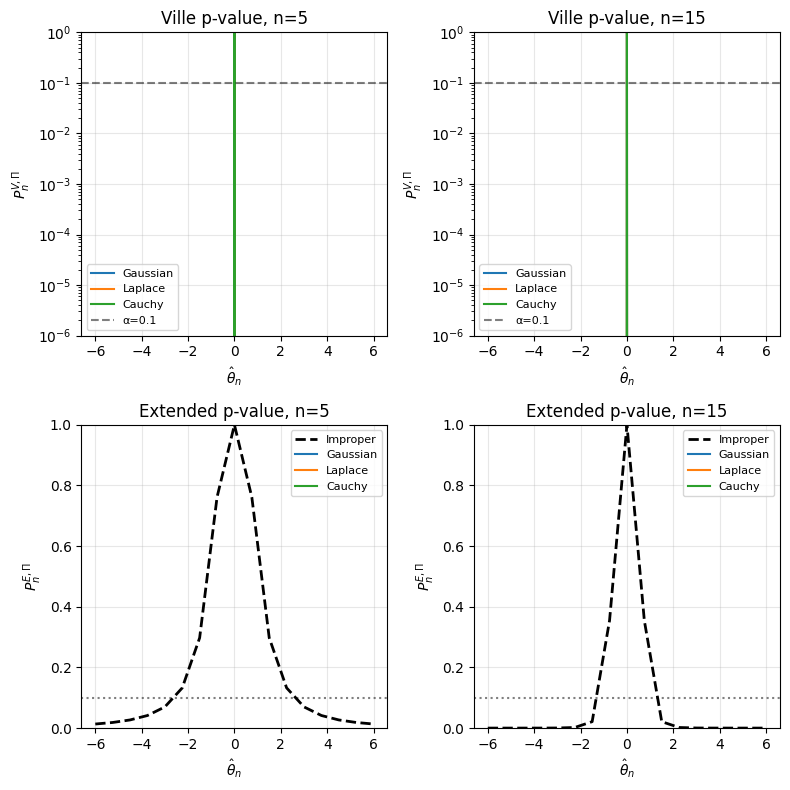
\includegraphics[width=0.5\linewidth]{images/output1.png}
    \caption{p-values as functions of $\hat{\theta}_n$. Ville p-values degenerate to $0$ as $|\hat{\theta}_n|$ increases extended p-values remain bounded}
    \label{image1}
\end{figure}

\subsection{Experiment $1$}
The experiment computes p-values as a function of $\hat{\theta}_n$ for fixed sample sizes $n$ (here $n=5, 15$) treating $\hat{\theta}_n$ as a free parameter ranging over a fixed range. For each $\hat{\theta}_n$, the scale invariant statistic $u_n = \frac{n\widehat \theta_n}{\sqrt{(n-1)+n(\widehat\theta_n)^2}}$ is computed and then both the Ville p-value $P_n^{V,\Pi} = \frac{1}{M_n^{\Pi}(u_n)}$ and the extended p-value $P_n^{E, \Pi} = g_{\mathrm{Leb}}(M_n^{\Pi}(u_n))$ are evaluated for three proper priors (Gaussian, Laplace, Cauchy) centered at $0$. Varying $\hat{\theta}_n$ away from $0$ simulates increasing data-prior conflict since the priors are centered at 0.

Figure \ref{image1} displays Ville and extended p-values as functions of the sample Sharpe ratio $\hat\theta_n$. The top row shows Ville p-values on a log scale. The bottom row shows extended p-values computed via the approximation $g_{\mathrm{Leb}}(M_n^{\Pi})$. 





\subsection{Experiment $2$}

\begin{figure}[ht]
    \centering
    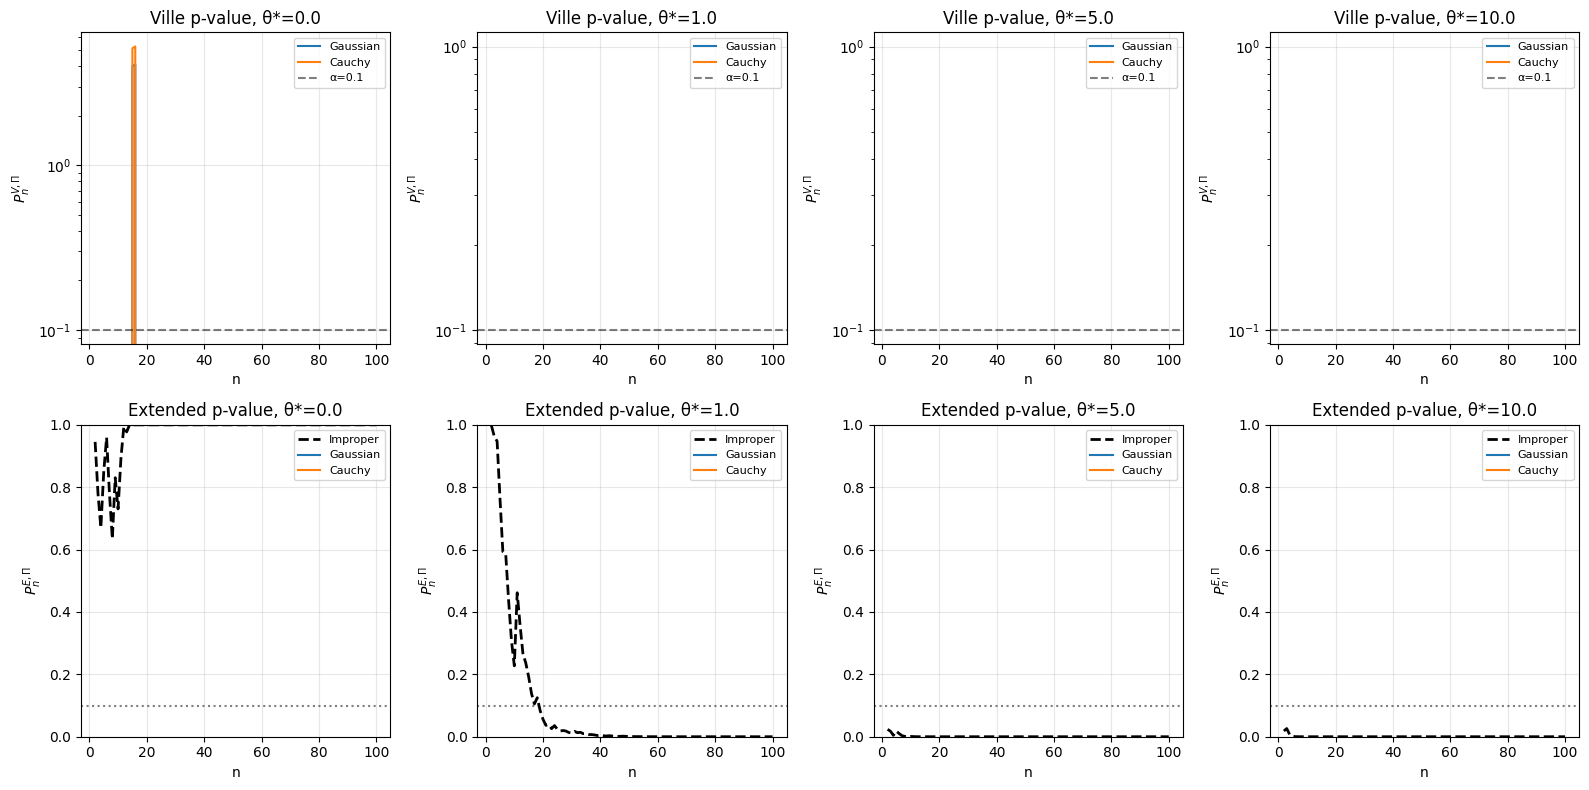
\includegraphics[width=\linewidth]{images/output2.png}
    \caption{p-value trajectories for priors centered at $0$. Ville p-values collapse immediately under conflict, extended p-values decrease gradually}
    \label{image2}
\end{figure}

The experiment generates a single realization of $Y_1, \ldots, Y_{100}$ from $N(\theta^* \sigma, \sigma^2)$ with $\sigma = 1$ and $\theta^* \in \{0, 1, 5, 10\}$, then computes running p-value trajectories as 
$n$ grows from $2$ to $100$. Priors (Gaussian, Cauchy) are centered at $0$, so increasing $\theta^\star$ corresponds to increasing data-prior conflict. Unlike Experiment $1$ which varied $\hat\theta_n$ deterministically, this experiment shows how p-values evolve with actual sequential data.

Figure \ref{image2} shows for $\theta^\star = 0$, Ville p-value fluctuate near $1$ for small $n$. We should be able to see Ville p-value going to $0$ immediately as mixture martingale explodes when data conflicts with the prior. Extended p-values should decrease gradually as evidence against $H_0$ accumulates, crossing the threshold $\alpha = 0.1$. The convergence should be faster for larger $\theta^\star$.


\section{Summary of Results}
We are testing 
$H_0:\theta^*=0 \text{ vs. }H_1:\theta^*\neq 0$ for normal data where both $\mu$ and $\sigma$ are unknown. The scale invariant statistic is used to construct mixture martingale under a prior $\Pi$. 

\paragraph{Proved Results:} 
\begin{itemize}
    \item Proposition \ref{prop:improper-Mn} ($\kappa = 0$) derives closed form for Lebesgue mixture $M_n^{\mathrm{Leb}}(u)
=
\sqrt{\frac{2\pi}{n}}
\left(1-\frac{u^2}{n}\right)^{-n/2}$
    \item Proposition \ref{prop:g-improper} ($\kappa = 0$) derives closed form for Lebesgue calibration $g_{\mathrm{Leb}}(c)
=
\E_0\!\left[\min\!\left(\frac{M_2^{\mathrm{Leb}}(Y_{1:2})}{c},1\right)\right]$. 
\item Theorem \ref{thm:recover-improper} ($\kappa = 0$) shows that the extended p-variable under a shifted polynomial-tail prior converges to the noninformative Lebesgue p-variable as data-prior conflict grows, ensuring robustness to prior misspecification.

\item Theorem \ref{thm:cs_vol} shows Ville CS volume diverges as $|\hat{\theta}_n| \to \infty$ for any proper prior. (Not sure if we should omit and only work with p-variables)

\item ($\kappa \geq 0$) derives closed form for $\kappa$-exponential mixture $M_n$ (like Proposition 2). 
\end{itemize}


\paragraph{Results we wish to prove:} 
\begin{itemize}
    \item ($\kappa \geq 0$) closed form for $\tilde{g}_\kappa$ does not exist. So no analog for Proposition 3. We can still maybe prove continuity, strict monotonicity, existence of inverse etc.

    \item We want to prove a theorem showing Ville p-value degeneracy i.e. $P_n^{V,\Pi_0}(y_{1:n}) \to 0$ as $|\hat\theta_n| \to \infty$. It should be obvious as $M_n^{\Pi_0}(u_n) \geq \int_0^\infty h_{\theta,n}(u_n) \pi_0(\theta) \, d\theta \to +\infty$
    \item Repeat the proof of everything for the case while testing $H_0:\theta^*=\theta_0 \text{ vs. }H_1:\theta^*\neq \theta_0$, where $\theta_0 \in \mathbb{R}$.
\end{itemize}


% $\kappa = 0$:
% \begin{equation}\label{eq_limit_fn}
%     \tilde{g}_\kappa (x) = \E \left[\min \left(x^{-1}\frac{h_2(U_2)}{h_{0,2}(U_2)}, 1\right)\right]
% \end{equation}
% where $U_2 = \frac{Y_1+Y_2}{\sqrt{Y_1^2 + Y_2^2}}$.

% \begin{proposition}
    
% \end{proposition}



\bibliography{bayesanytimettest}
\bibliographystyle{alpha}

\end{document} 